\documentclass[a4paper,12pt]{article}
\usepackage[a4paper, margin=1in]{geometry}  % You can change margin=1in to desired values
\setcounter{secnumdepth}{3}
\usepackage{comment}
\usepackage[usenames,dvipsnames,table]{xcolor}
\usepackage{pdfcolmk} 	% to correct pdflatex colour mistakes
\usepackage{cancel} %for strinking through terms which cancel oUa_1
\usepackage{fancyhdr}
\usepackage{placeins}
\usepackage{soul}
\usepackage{graphicx}
\usepackage{caption}
\usepackage{subcaption}
\usepackage{float}
%\usepackage{cite}
\usepackage{bm}
\usepackage{rotating}
\usepackage[utf8]{inputenc}
\graphicspath{{../results/}}  % figures live in the repo-level results/ folder
\usepackage{amsmath}
\DeclareMathOperator{\sign}{sign}
%\usepackage{natbib}%[aUa_1horyear,sort]
\usepackage{latexsym}
\usepackage{amssymb}
\usepackage{setspace}
\usepackage{amsmath}
\usepackage{framed} \definecolor{shadecolor}{cmyk}{0 0 0.2 0}
\usepackage{amsthm}
\newtheorem{definition}{Definition}
\newtheorem{proposition}{Proposition}
\newtheorem{theorem}{Theorem}
\newtheorem{example}{Example}
\newtheorem{corollary}{Corollary}
\newtheorem{lemma}{Lemma}
\usepackage{qtree}
\usepackage{makecell}
\usepackage{listings}

\lstset{
  language=Python,
  basicstyle=\ttfamily\small,
  keywordstyle=\color{blue},
  commentstyle=\color{gray},
  stringstyle=\color{orange},
  showstringspaces=false,
  breaklines=true,
  frame=single
}
\usepackage{setspace} 
\doublespacing
\usepackage{endnotes}

\let\footnote=\endnote

\usepackage[colorlinks,urlcolor=blue,citecolor=blue,linkcolor=blue,pdfstartview=FitH,pdfpagemode=UseNone]{hyperref}
\usepackage{rotating}
\usepackage{authblk}
\usepackage{orcidlink}
\usepackage[normalem]{ulem}
\newcommand{\del}[1]{\sout{#1}}
\usepackage{epigraph}
%\usepackage{natbib}
%\setcitestyle{square}

\usepackage[style=verbose, citestyle=numeric, bibstyle=numeric]{biblatex}
\addbibresource{1refs.bib}

\sloppy
\usepackage{tabularx}
\newcommand{\juergen}[1]{\textcolor{cyan}{#1}}
\newcommand{\ignacio}[1]{\textcolor{red}{#1}}
\newcommand{\new}[1]{\textcolor{magenta}{#1}}


\usepackage{lmodern}
\usepackage{graphicx}

\usepackage{tikz}
\usetikzlibrary{shapes,arrows,positioning, arrows.meta, quotes}
\usetikzlibrary{decorations.pathreplacing,shapes.misc,bending}
\usepackage{pgfplots}

\tikzset{decision/.style={diamond, draw, fill=blue!20, text width=4.5em, text badly centered, inner sep=0pt}}
\tikzset{block/.style={rectangle, draw, fill=blue!20, text width=5em, text centered, rounded corners,
 minimum width=3.5cm}}
\tikzset{line/.style={draw, -latex}}
\tikzstyle{process} = [rectangle, minimum width=3cm, minimum height=1cm, text centered, draw=black, fill=orange!30]
\tikzstyle{io} = [trapezium, trapezium left angle=70,minimum width=3cm, minimum height=1cm, trapezium right angle=110, text centered, draw=black, fill=blue!30]

\title{Vaccination Policy under Model Uncertainty: Can the Needs of the Few Outweigh the Needs of the Many? }


\author{
%\begin{comment}
\author[1]{\large J\"urgen Landes \orcidlink{0000-0003-3105-6624} \normalsize}
\author[2]{\large  Ignacio Ojea Quintana \orcidlink{0000-0001-6941-7283} \normalsize}
\affil[1,2]{Munich Center for Mathematical Philosophy, LMU Munich, 80539 Munich, Germany}
\affil[*]{Corresponding author's email: \href{mailto:juergen_landes@yahoo.de}{juergen\_landes@yahoo.de}}}
%\end{comment}

\allowdisplaybreaks
\begin{document}


\maketitle
\epigraph{The needs of the many outweigh the needs of the few.}{Spock, The Wrath of Khan}% \cite{Littmann2016}}
\begin{abstract}
Vaccination policy is often justified by appealing to epidemiological models suggesting that universal vaccination maximises public health and that vaccine refusal constitutes ethically blameworthy free-riding. We examine the robustness of these ethical inferences by developing an epidemiological model that incorporates an empirically motivated but often neglected feature: immunity declining virulence over successive transmissions. Our simulations establish the existence of parameter regimes in which vaccinating only a vulnerable subgroup results in fewer total deaths than vaccinating the entire population, even when vaccines are safe, effective, freely available, and rapidly deployable.

We do not claim that such conditions characterised COVID-19, nor that selective vaccination strategies are ethically preferable in general. Rather, our results demonstrate that ethically salient conclusions—concerning collective benefit, free-riding, or moral blame—can depend sensitively on modelling assumptions that are uncertain, contestable, and frequently under-specified in public discourse. We argue that this underdetermination supports a stance of epistemic humility in public health ethics, especially when epidemiological models are used to justify strong moral judgments about individual or group behaviour under conditions of deep uncertainty.
\end{abstract}

\noindent{\bf Keywords}: COVID-19; public health; trust in models; vaccination policy.

\juergen{To be cited: \cite{Iranzo2021}.}
%\href{https://drive.google.com/drive/folders/19CJT4v1UVg0fyVk9oToUTj3_4RKsZ5ya?usp=sharing}{GDrive Link}

\subsection*{Comments from Reading Group}
Hamed: Too much hedging. Some general hand-waving how the optimisation works could be added. THe precautionary principle material is unclear. Figures 3 and 4: too much white.\\
Boris: Hedging is reasonable. Random sampling to get an idea how prevalent the phenomenon is. Hedge utilitarinism in conclusions; some versions of the theory might recommend Strategy 1.\\
Adria: don't be so sure that our model can compete with the super advanced models. Tone DOWN last sentence of the first paragraph in the conclusions.\\ If the super advanced models actually do model viral ageing, then our toy model is a ``limiting case'' of their model. Our analysis thus serves as a robustness check -- which they can't run due to complexity blowing up. Our main point \emph{be careful!} still goes through.\\
Also: as long as Strat 1 is only marginally better than Strat 2, we can't really blame free-riders; in particular when vaccinations (likely) cause some adverse reactions.

\subsection*{Comments from David Teira}
The paper seems to have two parts. In the first one, we find an argument for sub-group vaccination; in the second-one, this argument is undermined by the uncertainty about the modelling assumptions. The problem, I'd say, is that this second part is already known (in the HPLS collection we edited on covid, the point was hammered time and again). So I am not sure about what I have learnt.

Actually, the section I liked most was 3.5, on the deaths each vaccination strategy could cause. Basically, because it rationalized an intuition I had: no politician will want to bear the costs if selective vaccination backfires. The question is whether that 10\% of additional deaths selective vaccination could cause is  good reason or not to justify universal vaccination as a default.

You pile up so many objections that a reader like me losses track of what you are arguing for. If the paper is just an argument for epistemic humility, maybe it's not much of a contribution. But if it had been focused more narrowly on which sort of situations would licence selective vaccination (is it just deaths? Is it about how to choose which vulnerable people we vaccine), I would have learnt more. 

\begin{comment}
\subsection*{Authors}

J\"urgen Landes and Ignacio Ojea Quintana at  Munich Center for Mathematical Philosophy, LMU Munich, Ludwigstr. 31, 80539 Munich, Germany, 
{juergen\_landes@yahoo.de} -- corresponding author, orcidID {0000-0003-3105-6624}, phone: +491632343319\\
Article type: Original Research\\
Running title: Vaccination Policy

\subsection*{Statements and Declarations}

\subsubsection*{Funding}
J\"urgen Landes gratefully acknowledges funding from the Deutsche Forschungsgemeinschaft (DFG, German Research Foundation)—project number 528031869.
\subsubsection*{Ethical approval}
No ethical approval was required since all data used is publicly available.
\subsubsection*{Informed consent}
Since all data used is publicly available, informed consent issues do not apply.
\subsubsection*{Author contribution}
All authors contributed to all stages of drafting this manuscript. All authors have read and agreed with the final version of the manuscript.
\subsubsection*{Data Availability Statement}
All real-world data used is publicly available.\\
The code for producing the simulated data is attached.

\subsubsection*{Competing Interests / Conflict of Interest Statement}
We do not have any competing interests.
%\end{document}
\end{comment}



\section{Introduction}\label{sec:Intro}
Public vaccination campaigns have enjoyed spectacular successes, such as the eradication of smallpox and the virtual eradication of tetanus and polio by achieving herd immunity \cite{Haelle2024}. These successes were used to argue that vaccination refusal constitutes free-riding or even harms public health and is thus ethically blameworthy \cite{Hoven2012,Giubilini2018}. The development of vaccines, which were widely effective against SARS-CoV-2 \cite{Altmann2022} and safe \cite{Sessa2021}, sparked heated ethical debates about free-riding, mandated vaccination, herd immunity, and the curtailing of personal liberties for non-vaccinated individuals in order to improve public health \cite{Graeber2021,Singer2021,Choy2022,ChuanVoo2022,Kelsall2024,Giubilini2020,Bernstein2023,Bradley2021,Williams2021a,Kraaijeveld2022}. The main argument of the pro-vaccination camp -- virtually unchallenged by opponents -- was that mass vaccination would surely improve public health.
\begin{quote}
Transmission models were used to devise vaccination strategies and served as a basis for policymaking in many countries$^{33,41–43}$. The model-based assessment of the vaccination impact incorporates biological characteristics of the virus, age-dependent effects in transmission and disease severity, epidemiological effects of vaccines, and additional factors that are setting-specific (e.g., the level of non-pharmaceutical interventions, vaccine supply, and SARS-CoV-2 seroprevalence prior to vaccination rollout$^{29}$). \cite[P.\ 3]{Rouzine2023} 
\end{quote}
In this paper, we critically examine the evidential basis for the claim that mass vaccination would surely improve public health. We show that in some Covid-19-like situations, it is overall preferable to vaccinate only a small subgroup of the population, namely those who are vulnerable. This is so, even though i) the vaccine causes no adverse reactions nor nocebo effects\footnote{The nocebo effect of a vaccination occurs when patient expectations (rather than the vaccine) worsen reported outcomes; just knowing that one has been vaccinated can make one feel badly.}, ii) the vaccine is freely available in unlimited quantities,  iii) distribution and vaccination are immediate, iv) the mortality rate of non-vulnerable people is greater among non-vaccinated than among the vaccinated (both are non-zero) and v) there is no change in (available) public health measures (social distancing, school closures, travel bans, air cleaners, mask availability, and quality). Even though non-vulnerable people are individually worse off (greater risks of infection and death) in situations considered here, the need to protect the vulnerable outweighs the health benefits of the non-vulnerable. Put differently, \emph{the needs of the few outweigh the needs of the many}, cf.\ \cite{Savulescu2020}.\footnote{Famously, the Star Trek character Spock calls it logical that instead \emph{the needs of the many outweigh the needs of the few} \cite{Littmann2016}. Spock's intuition is borne out in utilitarianism, if the amount of utility a member of the ``few'' sacrifices is equal to (or less than) the amount of utility a member of the ``many'' gains. However, if every member of the ``many'' sacrifices much less than a member of the ``few'' stands to gain, then utilitarianism can make it obligatory for the many to sacrifice utility to improve the lives of the few.}


Our argument fits within a wider philosophy of models in science and policy that has been calling for a reduction in the strength of conclusions one can justifiably draw from scientific theories and models in general \cite{Cartwright2016a} and Covid-19 models in particular \cite{Winsberg2024}. Unlike previous criticisms made on principled grounds and/or on concrete case studies, we instead identify a biological mechanism that is (mostly) missing in theories and models, which we integrate into our own model. Since our model seems no less reasonable than previous models and the results from our model conflict with the received wisdom, we argue that we should be very careful when drawing epidemiological and ethical conclusions from pandemic models. Unlike most previous work, our call for epistemic humility is rooted in a constructive approach.

The situation we describe and the model we build are motivated by the observation that flu viruses evolve(d) over time and became less deadly.
\begin{quote}
Prior respiratory pandemics showed development in waves and the pandemic phase extended over a 2–3 years course. The waves were characterized by different clinical severity and the pandemic phases seem to end with an attenuation of the viral virulence. [..] Even without efficient vaccines and drugs, the pandemic phase of the Russian and Spanish flu ended after a wave associated with milder symptoms.

It is, of course, a matter of conjecture whether we are with the omicron wave of COVID-19 in a comparable situation as the Spanish flu in 1920 and the Russian flu in 1892. The higher transmissibility and the lower virulence of omicron compared with the delta variant with a preferential replication in the upper over the lower respiratory tract are hopeful signs and correspond also to general ideas about the evolution of transspecies infections. There is thus hope that we might see in 2022 the end of the pandemic phase of COVID-19. \cite[P.\ 1314]{Bruessow2022} 
\end{quote}
And so it did come to pass: WHO Director-General TA Ghebreyesus declared on 5.5.2023 that Covid-19 is no longer a ``public health emergency of international concern'' \cite{WHO2023}. What exactly caused the end of the pandemic is hard to tell; vaccines are widely believed to have played a major role.

Although our model is clearly inspired by Covid-19, our aim is to build a generic model for studying epidemic dynamics that is relevant for future public health decision making \cite{Casadevall2024}. In order to avoid any possible confusion on this highly sensitive issue: our contribution is not a comment on actual (successes of) Covid-19 vaccination strategies. Furthermore, our investigation targets the assessment of vaccination strategies for populations and not individual behaviour. Consequently, claims concerning the moral status of individual actions could only follow as a corollary, which might require further substantive assumptions.

The rest of the paper is organised as follows: We next motivate and introduce our model (\S~\ref{sec:Model}), report our simulations in \S~\ref{sec:Results} and then deal with an objection in \S~\ref{sec:Objection}. \S~\ref{sec:Conclusions} discusses our results and offers some conclusions. The appendix provides some implementation details.

\section{The Model} \label{sec:Model}
We use an agent-based model to represent infection dynamics in a population. Agent-based models allow us to study phenomena emerging from (inter)actions of autonomous agents and to assess initially plausible, qualitative hypotheses about complex systems \cite{Casini2025a}. We next describe the most important modelled concepts and then provide implementation details.
\subsection{Main Components of the Model}

\paragraph{Base Model.} Our model is a discrete time \textbf{SISD model}, meaning that agents are initially susceptible (S) to infection (I), and an infection can have two mutually exclusive outcomes: either the agent eventually recovers and becomes susceptible again (S) or the agent dies (D). Agents are initialised in random locations on a two-dimensional grid, and their movements are described by a simple symmetric random walk where they are equally likely to go up, down, left or right. Whenever an infected agent and a susceptible agent occupy the same location, the susceptible agent is infected with some probability. Furthermore, at each time step, infected agents either die with some probability or have an increasing probability of recovery. Four features are added to this simple and standard setup.

{\bf 1. Vulnerable Agents.} We split the population of agents into two sub-populations, vulnerable and non-vulnerable agents, in order to capture that some people have much worse prospects than others, e.g., older patients \cite{Biswas2021} and immunocompromised patients \cite{Bytyci2024}. We make the following assumptions about vulnerable, ``high-risk'' agents. Vulnerable agents are more likely to become infected, more likely to die from an infection, and take longer to recover. These prospects are controlled by a parameter (see below).

{\bf 2. Immunity.} We also model that survivors of a Covid-19 infection build up immunity \cite{Hall2021}. Every time an infected agent recovers, it gains some immunity: it lowers their future infection probability, decreases their chance of dying once infected, and speeds up their recovery time.\footnote{The concept of immunity has recently been discussed in \cite{Zach2023}.}\

{\bf 3. Vaccination.} Covid-19 vaccines reduced the risks of (serious) infection and death \cite{Altmann2022,Rouzine2023}. In our model, vaccinated agents have a significant advantage over non-vaccinated agents in terms of infection probability, recovery time, and probability of death.

{\bf 4. Viral Age.} As mentioned in the introduction, we take into account that viruses change over time, for general considerations see \cite{Duffy2018} and \cite[P.\ 4]{Rouzine2023} for Sars-Cov-2.\footnote{Obviously, not all changes (mutations) in viruses make them more benign; some evolved sub-variants can have greater mortality rates, and some mutations are the actual cause of a wave, cf.\ \cite{Kun2023,Schroeder2023}. Effects of vaccinations on virulence are investigated in \cite{Gandon2001}. See \cite{Sanjuan2016} for a review of biological mechanisms of virus mutation, \cite{Lauring2013} for theoretical underpinnings, and \cite{Jones2024} for concrete in silico models.} We here implement a version of the  transmission–virulence trade‑off hypothesis:
\begin{quote}
In plain words, if a pathogen causes its host to lay in bed or even to die instead of happily going around and transmitting the infection, it will be outcompeted by mutants that cause less damage to the host and allows it to produce more pathogens and infect other hosts. \cite[P.\ 71]{Kun2023} 
\end{quote}
In our model, the viral age of a virus increases by one every time a virus infects (jumps) from an infected agent to a susceptible agent. Lethality decreases with viral age (transmission–virulence trade-off), while transmission probability\footnote{The simulation study \cite[P.\ 1]{Saldana2024} instead finds that ``variants with milder symptoms are likely to spread faster than those with severe symptoms. This is because severe variants can prompt affected individuals to seek medical help earlier, potentially leading to quicker identification and isolation of cases. However, milder or asymptomatic cases may spread more widely, making it harder to control the spread.''} and recovery time remain constant. Infection dynamics of our model are sketched in Figure~\ref{fig:Flowchart}.

All core elements of the model are drawn from established epidemiological approaches; our aim is not to introduce new modelling techniques, but to explore their consequences.

\begin{figure}
\begin{center}
\scalebox{0.6}{
      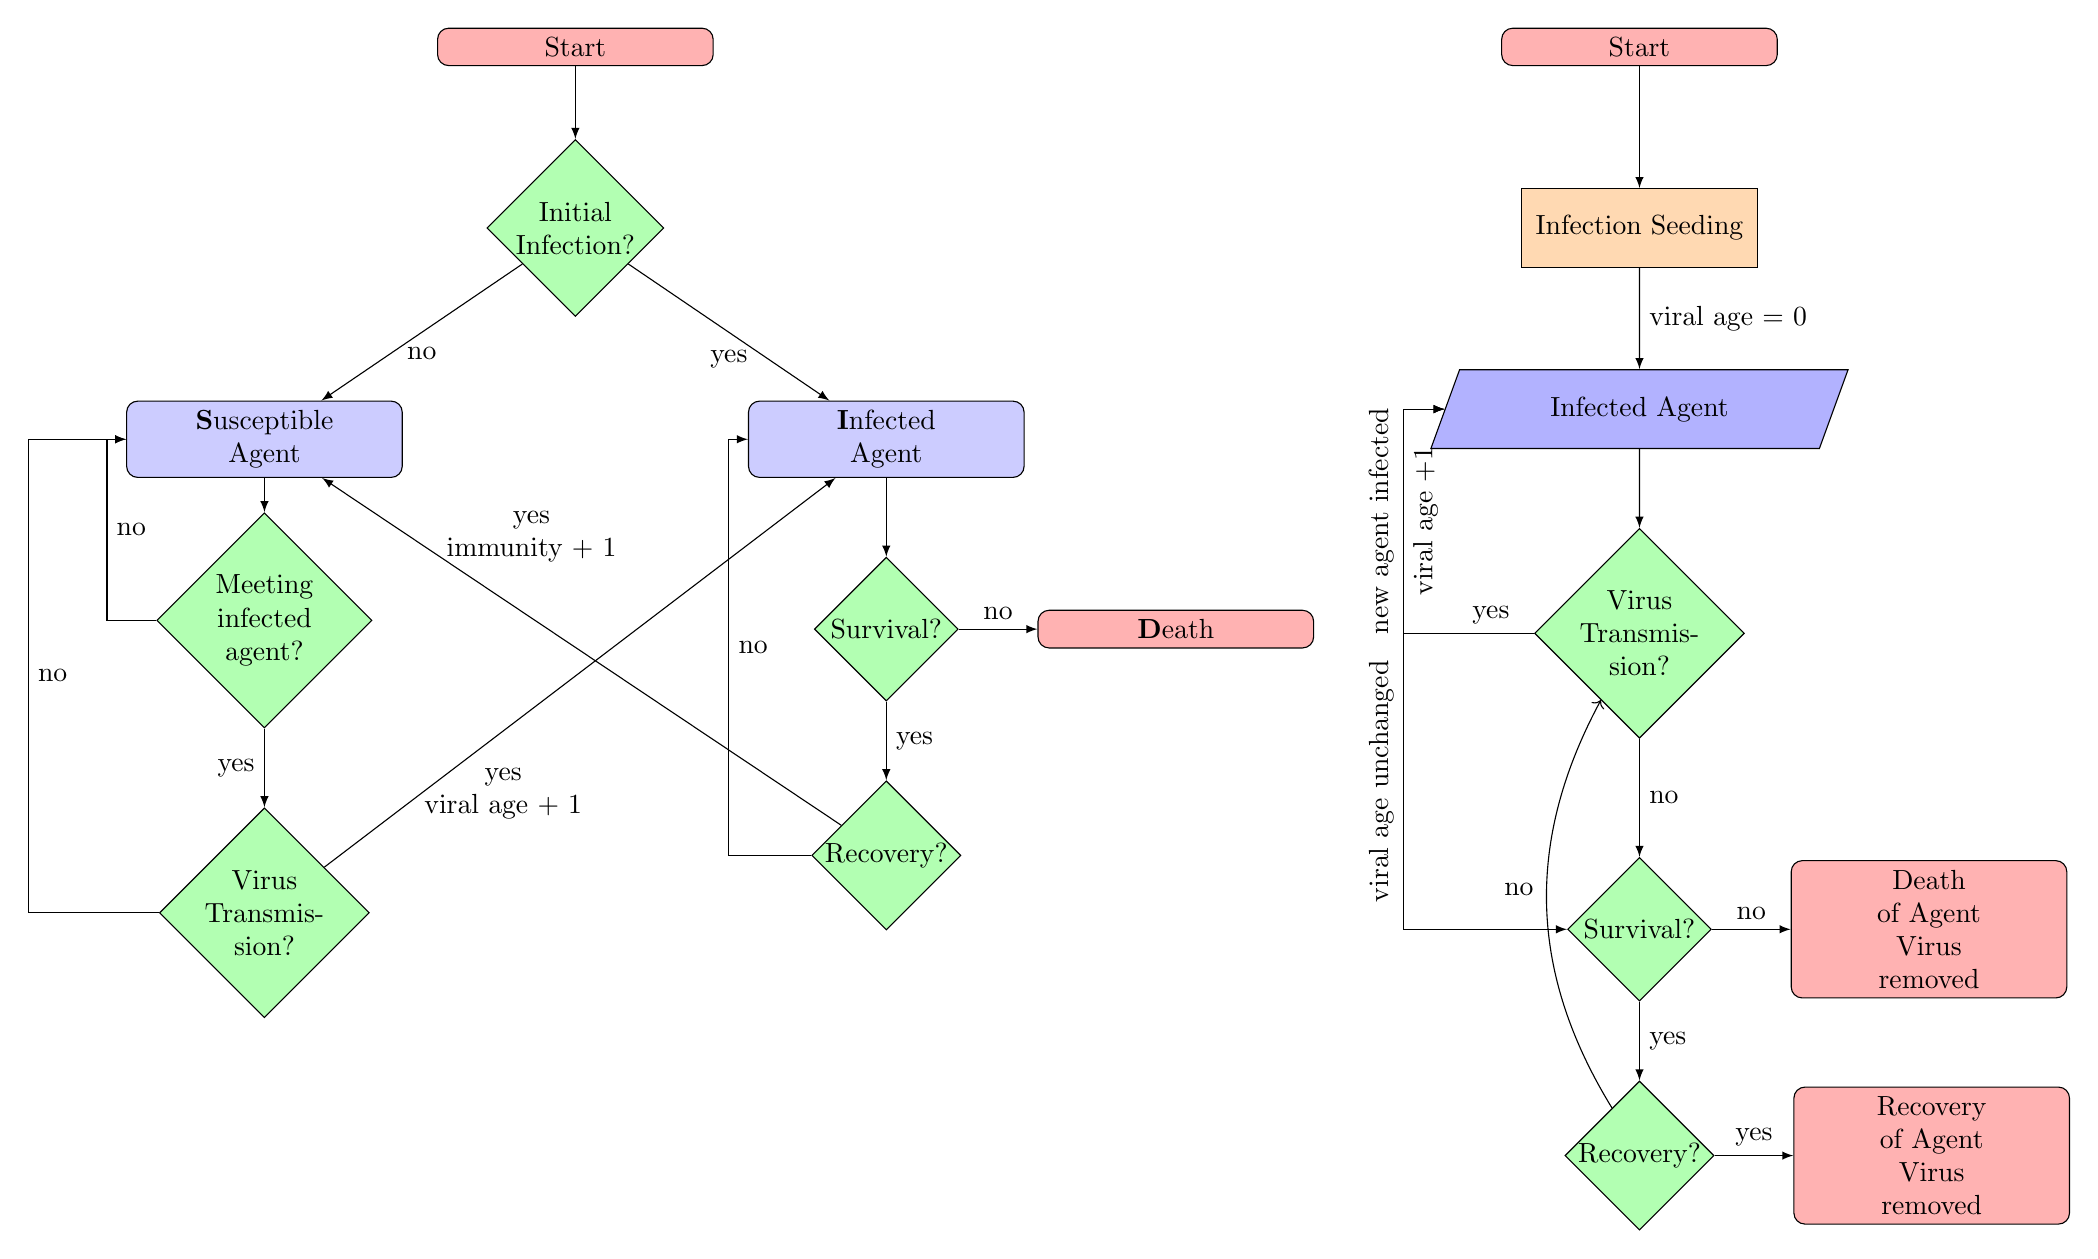
\begin{tikzpicture}[node distance=2.3cm]
        \node[block, fill=red!30]                  (init){Start};
        \node[decision, below of=init, fill=green!30]   (Inf){Initial Infection?};
        \node[block, below left = of Inf]   (Infno){{\bf S}usceptible Agent};
        \node[block, below right = of  Inf](InfYes){{\bf I}nfected Agent};
        \node[decision, below of=Infno, fill=green!30]   (Meet){Meeting infected agent?};
        \node[decision, below =1cm of Meet, fill=green!30]   (Inf2){Virus Transmission?};
        \node[decision, below =1cm of InfYes, fill=green!30]   (Sur){Survival?};
        \node[decision, below =1cm of Sur, fill=green!30]   (Rec){Recovery?};
        \node[block, right =1cm of Sur, fill=red!30]   (DD){{\bf D}eath};
        \path[line] (init) --          (Inf);
        \path[line] (Inf) --  node[below,yshift=-2pt]{no}        (Infno);
        \path[line] (Inf) --   node[below,yshift=-3pt]{yes}  (InfYes);
        \path[line] (Infno) --          (Meet);
        \path[line] (Meet) --   ++(-2,0) |- node[pos=.25, right]{no}  (Infno);
        \path[line]  (Meet) -- node[left]{yes} (Inf2);
\path[line] (Inf2) -- node[pos=0.35, below, yshift=-10pt, align=center]{yes\\viral age + 1} (InfYes);
        \path[line] (Inf2) --   ++(-3,0) |- node[pos=.25, right]{no}  (Infno);
        \path[line] (InfYes) --          (Sur); 
\path[line] (Rec) -- node[pos=0.65, above, yshift=10pt,xshift = 10pt, align=center]{yes\\immunity + 1} (Infno);
        \path[line] (Sur)--node[right]{yes} (Rec);
        \path[line] (Rec) --  ++(-2,0) |- node[pos=.25, right]{no}  (InfYes);
        \path[line]  (Sur) -- node[above]{no} (DD);      
       \node[block, fill=red!30, right = 10cm of init]        (S){Start};
       \node (Ini) [process, below of=S] {Infection Seeding};
\node (Inf) [io, below of=Ini] {Infected Agent};
\node[decision, below =1cm of Inf, fill=green!30]   (T){Virus Transmission?};
\node[decision, below = 1.5cm of T, fill=green!30]   (Sur){Survival?};
\node[block, right =1cm of Sur, fill=red!30]   (DD){Death of Agent Virus removed};
\node[decision, below =1cm of Sur, fill=green!30](Rec){Recovery?};
\node[block, right =1cm of Rec, fill=red!30]   (D){Recovery of Agent  Virus removed};
\path[line] (S) --(Ini);
\path[line] (Ini) -- node[right]{viral age = 0} (Inf);
\path[line] (Inf) --(T);
\path[line] (Sur) -- node[above]{no} (DD);
\path[line] (Sur)--node[right]{yes} (Rec);
\path[line] (Rec) -- node[above, align=center]{yes} (D);      
\path[line] (T)--node[right]{no} (Sur);
\path[line] (T) --   ++(-3,0) |- node[pos=.25, right, rotate = 90,above]{new agent infected}  (Inf);
\path[line] (T) --   ++(-3,0) |- node[pos=.25, right, rotate = 90,below]{viral age +1}  (Inf);
\path[line] (T) --   ++(-3,0) |-node[pos=0, right, above]{$\quad\quad\quad\quad\quad\quad$ yes}   (Inf);
\path[line] (T) --   ++(-3,0) |- node[pos=.25, right, rotate = 90,above]{viral age unchanged}  (Sur);
\path (Rec) edge[->, bend left]
    node[pos=0.5, above, xshift=-10 pt]{no} (T);
\end{tikzpicture}
}      
\end{center}
\caption{Schematic flowchart representation of infection dynamics in our model. The figure on the left captures the population of agents, the figure on the right captures dynamics of viral ageing and omits non-infected agents. The probabilities governing the green decision nodes are specified in the text, which depend on the type of the agent (vulnerable or not) and on the immunity level of the agent (not represented here in full detail). Right figure: if a virus is transmitted, then two things happen: 1) a new agent is infected with a virus that has an increased viral age and 2) the viral age remains unchanged in the originally infected agent. This is represented by the bifurcated arrow.}
\label{fig:Flowchart}
\end{figure}

\subsection{Vaccination Strategies}
Having described the model, we can now consider vaccination strategies within our model. We here consider two vaccination strategies (a central planner of) a country might pursue. Since vulnerable people face dire consequences if infected, vulnerable agents are vaccinated in both strategies.
\begin{description}
\item Strategy 1: All agents are vaccinated.
\item Strategy 2: Only the vulnerable agents are vaccinated.
\end{description}
Our goal is to show that implementing \emph{the second strategy can lead to fewer dead agents than the first strategy} -- in some region of the parameter space. 

\paragraph{Qualitative Working Hypothesis}
We now attempt to explain how it might happen that Strategy 2 has fewer dead agents than Strategy 1. We make two key assumptions:
\begin{enumerate}
    \item Non-vulnerable, non-vaccinated agents are very unlikely to die.
    \item A vaccinated agent has a much smaller probability of being infected than a non-vaccinated agent -- ceteris paribus.
\end{enumerate}
Let us compare how Strategies 1 and 2 will likely impact simulations. Strategy 1: since all agents are vaccinated, it takes many more rounds before the virus ages and becomes sufficiently benign. Strategy 2: the virus mainly circulates among the non-vaccinated (Assumption 2), where it quickly becomes benign. This leads to an increase in infected agents, which are rather unlikely to die (Assumption 1).\footnote{The ``increased transmissibility of milder variants can still result in higher hospitalizations and fatalities due to widespread infection.'' \cite[P.\ 1]{Saldana2024}} However, since the virus circulates more in Strategy 2, it becomes more benign much faster than in Strategy 1.\footnote{Furthermore, as the virus circulates more, agents gain immunity faster; but this is not necessary for the possibility discussed here.} A benign virus in a non-vaccinated agent can, in principle, be less deadly than a non-benign virus in a vaccinated agent. So, \emph{it is possible} that Strategy 2 has fewer average deaths than Strategy 1.


This explanation attempt is, of course, not built on logically valid arguments, but rather on somewhat plausible steps of reasoning. Which of the two strategies actually performs better (in some region of the parameter space), we cannot determine before running a simulation.

\subsection{On Evaluation Metrics}
Our main evaluation metric for vaccination strategies is admittedly rather simplistic, as it depends only on a single number: the number of deaths. This metric can only be a first approximation. Firstly, the idea that all deaths are equally bad has been challenged, and quantification measures have been put forward \cite{Schwappach2002}. Secondly, how well other objectives of vaccination strategies are met, such as the minimisation of i) the economic burden, ii) the duration and iii) the total number of infections, as well as keeping the health system functional at all times \cite{Rouzine2023} are not taken into account by our metric.\footnote{Rouzine \& Rozhnova also argue that mass vaccination can have another related, unexpected and possibly unwelcome consequence: it accelerates the evolution of pathogens.}

Despite the oversimplification of the metric, the comparison of vaccination strategies using it raises important ethical questions for public policy [Who to vaccinate? Mandate vaccinations?] and the epistemology of (epidemiological) models [When can we believe in a model's prediction?].

In order to broaden the scope of evaluation, we also visualise the effect that the two strategies have on infections (infection rate times duration). This is called \emph{the area under the curve (AUC)}, since it can be calculated as the area under (integral over) the infection curve across time; see Figure~\ref{fig:AUC_and_deaths}.

Although this paper focuses on the number of deaths, other evaluation metrics could easily be used for assessments of vaccination strategies since our model and the code are relatively simple and thus malleable. For example, we also report AUC, exemplary further easy to implement metrics are: time steps until the last death (proxy for the duration of the pandemic), [maximal] number of infected agents at every step (a large number of infected agents at any given time can trigger the collapse of the health system), deaths and/or infections in geographical regions, and the number of virus transmissions (mutations).\footnote{To facilitate further applications, our simulation also outputs the number of times agents have been infected, the total number of infections, and the total number of infections of vulnerable and non-vulnerable agents.}

\subsection{Limits of Ethical Inference from the Model}\label{subsec:EthicalLimits}
It is important to be explicit about what kinds of ethical conclusions our model does and does not support. The simulations reported in Section~\ref{sec:Results} establish the existence of parameter regimes in which vaccinating only a vulnerable subgroup leads to fewer total deaths than vaccinating the entire population, given the evaluation metric adopted here. This result alone does not determine which vaccination strategy is ethically preferable, nor does it license direct policy recommendations.

First, our evaluation metric focuses exclusively on mortality and abstracts away from other ethically relevant dimensions, including morbidity, long-term health effects, distributional fairness beyond vulnerability status, economic costs, and constraints on individual liberty. Different ethical frameworks will weigh these dimensions differently, and reasonable disagreement about their relative importance should be expected.

Second, the ethical significance of our results depends on modelling assumptions that are themselves uncertain and contestable, including assumptions about viral evolution, immunity accumulation, and behavioral responses. Our model is intended as a constructive counterexample rather than as a realistic predictor of outcomes in any particular pandemic context.

Finally, our analysis targets population-level vaccination strategies rather than the moral evaluation of individual actions. Claims about individual responsibility, free-riding, or blameworthiness do not follow directly from the model and require additional normative premises that lie outside its scope.

Taken together, these considerations support a stance of epistemic humility: even when epidemiological models are internally coherent and empirically motivated, the ethical conclusions drawn from them may remain substantially underdetermined.

Because vaccination policy remains a highly polarising public issue, it is important to clarify how our results should be understood. Nothing in this paper implies that vaccination campaigns during the COVID-19 pandemic were ethically mistaken, unjustified, or harmful on balance, nor that vaccine refusal is ethically permissible or advisable. Our model is not intended to describe COVID-19 or to support selective vaccination as a general policy recommendation. Rather, it serves as a constructive counterexample demonstrating that, even under favourable assumptions about vaccine safety and efficacy, ethically salient conclusions about collective benefit, free-riding, or moral blame can depend sensitively on modelling choices that are uncertain and contestable. The purpose of the model is therefore epistemic rather than prescriptive: to show why strong moral conclusions drawn directly from epidemiological models should be treated with caution under conditions of deep uncertainty.

\subsection{Simplifications}\label{subsec:Simple}
Our model makes a number of clearly unrealistic, simplifying assumptions, such as the grid-based environment and the random movement dynamics; see also Table~\ref{tab:Simplifications}. For example, the model does not allow symptomatic agents to self-isolate; the probability of transmission, hence, does not depend on whether the infected agents have symptoms. Most of these simplifications could be easily replaced by further complicating the model. We are certain that more complicated versions of our model will yield quantitatively different results. For example, adding fatal adverse reactions to the vaccine to the model (which rarely occurred during Covid-19 \cite{Sessa2021}) would result in more deaths for the universal vaccination strategy than for Strategy 2, thereby strengthening our findings.

%We want to emphasise the effect of viral ageing and immunity growth as the key features of our model.

Real-world ethical assessments for policy-making must account for multiple dimensions of harm, including mortality, morbidity, economic impact, and long-term health, as well as issues of transparency and informed consent.

Despite all these simplifications, we are confident that the main qualitative conclusions our model licences can also be drawn from modified models and/or evaluation metrics.

%\begin{quote}
%The ``transmission–virulence trade-off,'' suggests that highly deadly viruses, such as Ebola, often kill their hosts rapidly, thereby reducing the chances of spreading to others (79). This tradeoff implies that viruses with high lethality tend to have lower transmission rates because the severe symptoms incapacitate the host and limit their interactions with others. Additionally, severe symptoms and higher mortality will often lead to people staying home, reducing the opportunity for the virus to spread. \cite[P.\ 6]{Jones2024}
%\end{quote}

\section{Simulation}\label{sec:Results}
\subsection{Set up}
Our main interest is to determine whether there are situations in which it is preferable not to vaccinate the entire population. In order to do this, we implemented an optimisation process to explore the parameter space, using \textit{scikit-optimize} \cite{head_scikit_optimize_2021}. For simplicity, we kept the parameter values stated above fixed and only varied three parameters: \emph{Viral ageing} in [0.1,0.9], \emph{Vaccination effect} in [0.1,0.9] and \emph{Death probability} in [0.01,0.9]. 

\subsection{Strategy 2 causes fewer Deaths than Strategy 1}
The goal is to find a set of parameter settings in which the difference in deaths between Strategy 1 (vaccinate all) and Strategy 2 (vaccinate vulnerable only) is positive (and maximal). For every parameter setting, we created $n=200$ random seeds, which specified the starting positions of all agents, whether they are vulnerable or not, and all other random numbers. The result of this optimisation process is plotted in Figure~\ref{fig:parameters}. The simulation is not intended to suggest that such parameter regimes are common; instead, it establishes that a variety of such regimes exist. Furthermore, these regimes are not confined to a tiny parameter range; rather, they are dispersed throughout the parameter space.

\begin{figure}[h!]
  \centering
  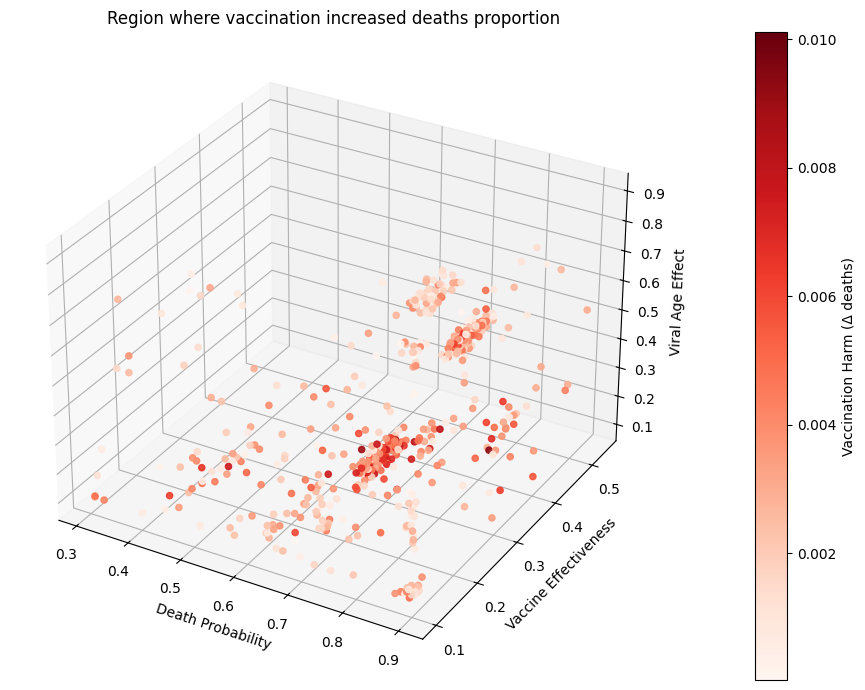
\includegraphics[width=0.70\textwidth]{vax_hurts.png}
  \caption{224 parameter settings where vaccinating all agents is worse with respect to deaths proportions. Colour-grades represents the (200-run) average difference between the proportion of deaths resulting from vaccinating all versus vaccinating vulnerable only.}
  \label{fig:parameters}
\end{figure}

The main results of these simulations are plotted in Figure~\ref{fig:parameters}. We note that i) the average difference between the strategies is never large (the maximal difference in proportions of dead agents is 1\% on average), and ii) the parameter region of interest is spread, and there does not seem to be any systematic relation between the parameters for which Strategy 2 was better than Strategy 1. These findings, we believe, strengthen our two (non-independent) points:
\begin{enumerate}
\item It is not trivial to predict when vaccinating everyone is the better strategy.
\item It is hard to be sure that Strategy 2 is worse in a specific situation.
\end{enumerate}

\subsection{Interpretation}
The emerging ethical picture is somewhat unusual. In order to achieve the greatest good for the entire population of agents in the model (measured by the lowest number of total deaths), it is sometimes preferable for a majority to increase their individual risks of infection and death(!) in order to confer a net benefit to the entire group. That is, getting vaccinated (sometimes!) lowers the utility of the population of agents in the model. Instead of unethical free-riding, foregoing vaccination is--in such situations--paradoxically an action that performs a public service by allowing the virus to attenuate in a low-risk population and thereby increasing the survival chances of the other agents. Ethically blameworthy free-riding thus turns into providing a public service, which carries substantial risks for the agent foregoing vaccination.

This situation can be understood as a sort of \emph{negative herd immunity effect}, where herd immunity may have negative consequences for those who remain susceptible \cite{Luyten2011}. A majority has a slightly increased probability of death, while a small minority has a strongly decreased probability of death. The expected net result is a reduction in deaths. At times, the needs of the few can outweigh the needs of the many -- if calculated by simple averaging. \cite{Luyten2011} discussed equity problems arising for vaccination policy due to a negative herd immunity effect, where negative effects occur since vaccinated individuals are initially protected from a pathogen but tend to fall seriously ill at an older age. The negative herd immunity effects discussed here do not depend on age but rather on the spread of the pathogen in the population.

\subsection{Area under the Curve}
As mentioned above, we also considered the area under the curve. Figure~\ref{fig:AUC_and_deaths}(left) shows the parameter settings for which Strategy 2 had a smaller area under the curve. Figure~\ref{fig:AUC_and_deaths}(right) shows the parameter settings for which Strategy 2 was better on average with respect to both AUC and the average proportion of deaths. These plots suggest that i) sometimes vaccinating all can be detrimental not only with respect to lives saved but also for proxies for economic burden, and ii) fewer deaths do not entail a smaller AUC. So even when we account for morbidity, there are regions of the parameter space in which universal vaccination decreases public health.

\begin{figure}[H]
  \centering
  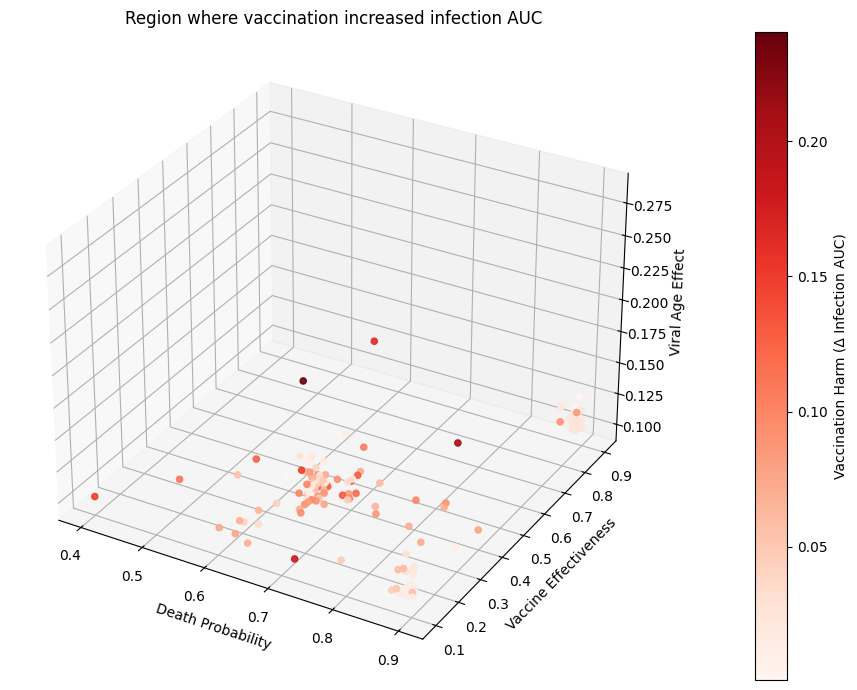
\includegraphics[width=0.45\textwidth]{AUC_vax_hurts.png}
  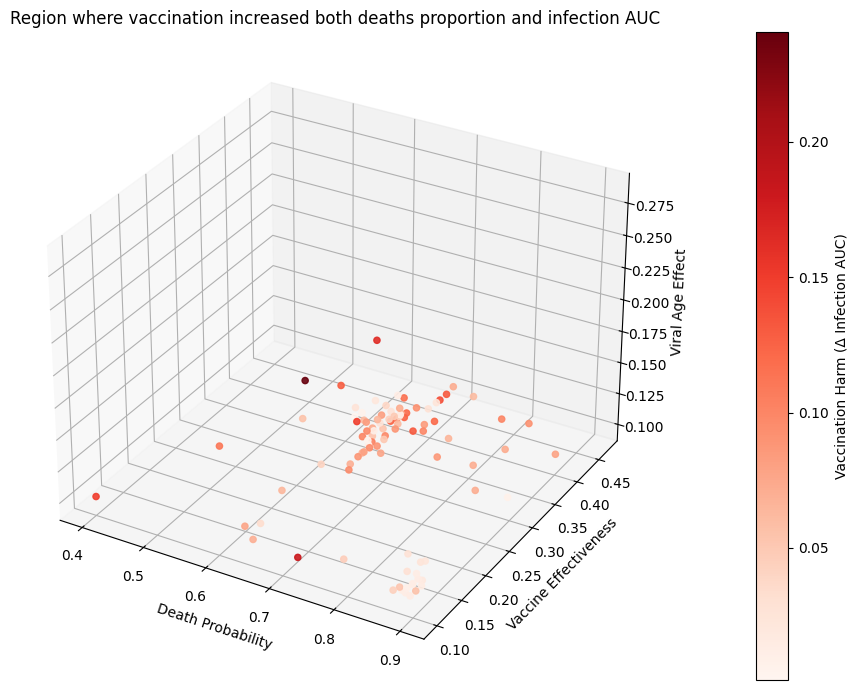
\includegraphics[width=0.45\textwidth]{ALL_vax_hurts.png}
  \caption{Colour-grades represent the (200-run) average AUC difference between the two strategies. Left: Parameter Settings where vaccinating all performed worse with respect to the area under the curve of infection. Right: Parameter Settings where vaccinating all performed worse with respect to i) deaths and ii) the area under the curve of infection.}
  \label{fig:AUC_and_deaths}
\end{figure}

Finally, Figure~\ref{fig:WhoGains} illustrates which group gains more from opting for Strategy 2 (regarding deaths), if Strategy 2 causes fewer deaths (224 parameter settings). For most parameter settings, both groups of agents are better off with Strategy 2 (first quadrant, top right in Figure~\ref{fig:WhoGains}). Most of the gains were for the vulnerable agents, which are represented as those parameter settings above the red diagonal. Furthermore, there are many parameter settings in the second quadrant (top left, negative $x$-coordinate). For these parameter settings, the group of non-vulnerable agents suffered more deaths under Strategy 2 than under Strategy 1, even though the opposite was true for the group of vulnerable agents. There are thus a number of parameter settings in which a majority group (non-vulnerable agents) sacrificed utility, resulting in much improved utilities for a minority (vulnerable agents) conferring a net benefit to the entire population. The needs of the few did outweigh the needs of the many.

\begin{figure}[H]
\centering
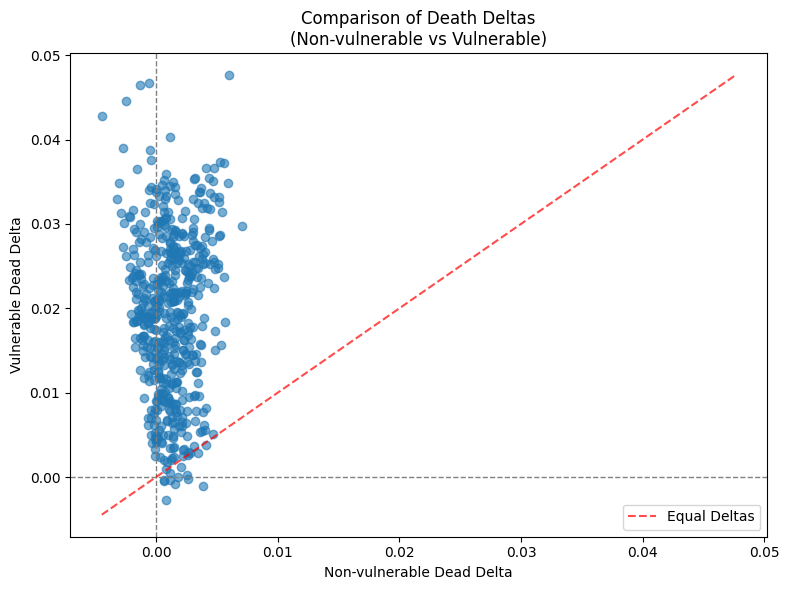
\includegraphics[width=0.70\textwidth]{vul_vs_nonvul.png}
\caption{Each dot corresponds to one of the 224 parameters settings found by the optimisation. The $x$-axis represents the advantage of Strategy 2 over Strategy 1 for non-vulnerable agents. The $y$-axis represents the advantage of Strategy 2 over Strategy 1 for vulnerable agents. Where $x<0$ and $y>0$ (top left) the relative dis-utility of the non-vulnerable agents is exceeded by the utility gain of the vulnerable agents -- \emph{the needs of the few outweigh the needs of the many.}}
\label{fig:WhoGains}
\end{figure}

\subsection{Worst Cases}
The Precautionary Principle and \emph{Primum non nocere} call for the avoidance of harms. One way to interpret harm avoidance is to avoid terribly bad outcomes as much as possible. In our setting, this can be translated into a reason for adopting the vaccination strategies that result in the fewest deaths in the worst case. The working hypothesis is as follows: vaccination of a small minority can lead to disastrous consequences that do not occur with universal vaccination. For both vaccination strategies, we hence \emph{independently} searched the parameter space for parameter values \emph{maximising} total deaths using the optimisation procedure described above [200 random seeds per parameter setting]. Figure~\ref{fig:WorstCase} indeed shows that the worst cases for universal vaccination have fewer deaths than the worst cases for selective vaccination. The difference in worst case deaths between these strategies is perhaps less than initially expected. Furthermore, there are many parameter settings in which Strategy 2 leads to more deaths than Strategy 1 causes in the worst case. Strongly harm averse decision makers confronted with deep uncertainty may hence rationally opt for Strategy 1.

\begin{figure}[H]
\centering
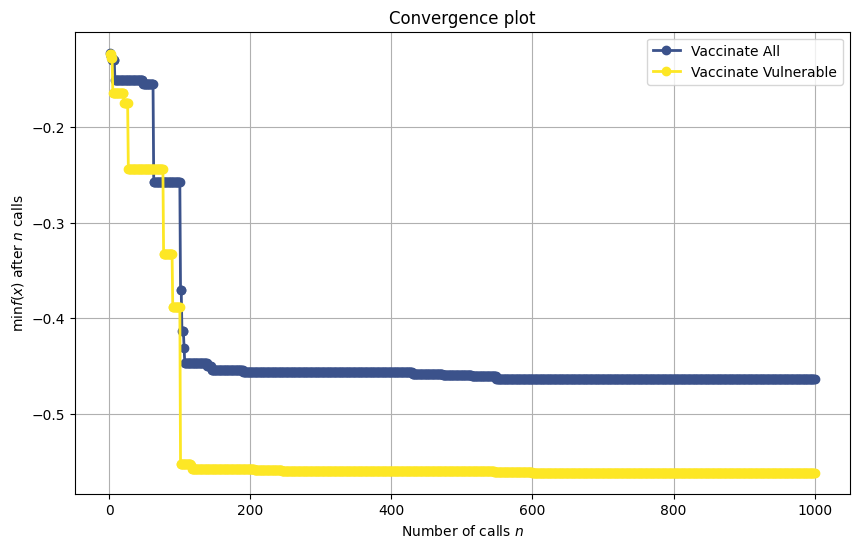
\includegraphics[width=0.80\textwidth]{Cropped.png}
\caption{Dynamics of maximisation of total deaths [200-run averages], $x$-axis: run number, $y$-axis: population decrease. Approximate maxima are obtained within the first 175 parameter settings. Universal vaccination (blue) caused at most 47\% agents to die, for selective vaccination the maximum was 56\%.}
\label{fig:WorstCase}
\end{figure}

\section{Model Appropriateness}\label{sec:Objection}
Before concluding, we address one objection: the existing Covid-19 models all pointed towards the public health benefits of universal vaccination, why should we care about the prediction of this ``speculative model''? Firstly, we acknowledge the broad agreement of existing models. Secondly, our model is less sophisticated than competing epidemiological models. Thirdly, the counter-intuitive result in our model only obtains for certain parameter values. If these parameter values do not approximate a concrete application, then our model also supports universal vaccination.

We want to resist the objection in several ways. Firstly, our model arose out of debates during the last pandemic; our stated aim is not to model Covid-19 but to be of use in the future. Failing to approximate parameter values for Covid-19 thus has direct implications only for the last pandemic and not for future ones. Secondly, simplicity is not necessarily a flaw, as it permits a better understanding than large black-box models and also facilitates robustness checks. Thirdly, the agreement of previous models could possibly be due to the fact that they all missed a crucial mechanism and are hence all misguided  . Fourthly, the existence of a single model speaking against universal vaccination raises the uncomfortable possibility of a multitude of such models. Instead of dismissing our anomalous model as noise, we believe that we ought to treat it as a reminder of the inherent unpredictability of human (public) health.

Finally, we want to point to historical precedents of vaccines leading to negative evolutionary outcomes. The case of Marek's Disease demonstrates how reducing host mortality without stopping transmission can inadvertently select for higher virulence \cite{Read2015}. Similarly, Pneumococcal conjugate vaccines (PCV) targeted the most common serotypes of Streptococcus pneumoniae. Previously rare, non-targeted serotypes quickly filled the ecological void. Some of these emerging strains have proven to be more antibiotic-resistant or more likely to cause invasive disease than the ones they replaced \cite{Hanquet2022}. These precedents suggest that our claim that selective vaccination might, in some regimes, lead to better outcomes is not merely a computational possibility but instead aligns with observed biological risks.

To improve our responses to future pandemics, we therefore suggest that the possibility of negative evolutionary outcomes be taken into serious consideration. This may include a duty to model the viral age and transmission-virulence trade-offs in order to avoid a model built on incomplete biological assumptions. Modelling further biological assumptions results in even more complex models, rendering them more opaque and hard to perform robustness analysis on. There are thus complicated trade-offs to be struck between model completeness on the one side and transparency and robustness of models on the other side.

\section{Conclusions}\label{sec:Conclusions}
Public health decisions, in particular those intended to combat a pandemic, are high stakes and fraught with uncertainty. During the Covid-19 pandemic, strong arguments were made for and against the use of vaccines and the implementation of vaccination strategies mandating vaccination (of subgroups). Some of these arguments (implicitly) build on an expectation that mass vaccination strategies would considerably improve public health \cite[P.\ 3]{Rouzine2023}. We developed a model that incorporates the well-documented feature of viruses, namely that their deadliness decreases over time, as well as an immunity build-up in agents. We believe that our model is a reasonable, yet clearly idealised, representation of an infectious disease such as Covid-19. Furthermore, we believe that relaxing or dropping idealisations will not simplify the task of finding optimal vaccination strategies. Existing models are more sophisticated in various ways because they also model host variability, long Covid, and population clustering. However, our model is more sophisticated with respect to virus mutation. It is therefore difficult to know a priori which model makes the best predictions.

Our model represents the transmission–virulence trade-off hypothesis. Whether this hypothesis is justified for Covid-19 has been challenged \cite{Kun2023}. With hindsight, we side with \cite{Bruessow2022} thinking that the hypothesis applies to Covid-19. Be that as it may, it is not immediately obvious whether this hypothesis will apply in future health emergencies. This kind of uncertainty makes the decision of whether to include the model of the transmission–virulence trade-off hypothesis an awkward one. This kind of uncertainty regarding what a proper epidemiological model should look like is an important reason why one should be cautious when drawing conclusions for public health from epidemiological models.

Taking into account the further, well-known difficulty of performing sensitivity analysis on epidemiological models (including our own) \cite{Edeling2021}, we hence argue that our understanding of the consequences of vaccination strategies is -- in many situations -- too poor to support strong arguments either way. We should hence be more careful before confidently labelling vaccine hesitancy as unfair free-riding, a boon, or simple negligence. 

While utilitarianism licences our main claim that vaccinating a selected minority is preferable to vaccinating the entire population (given certain assumptions), ethical pluralism strengthens our main argument. Since different ethical stances (towards the distribution and importance of harms and benefits of vaccination strategies) will, in general, make different judgments about the ethical desirability of vaccination strategies; other ethical theories might licence the negation of our claim. We feel that this divergence of assessments strengthens our call for epistemic humility.

Public health decision makers hence have the unenviable job of making high-stakes decisions fraught with uncertainty, complicated by conflicting advice from formal models. Although we have no strategy to offer here on how to make such decisions, we believe that part of any reasonable strategy are: i) epistemic humility and ii) good uncertainty communication when publicly announcing decisions \cite{Nutbeam2020,Intemann2023,Nguyen2024,Friedman2023,OjeaQuintana2021}. In particular, it is worth mentioning the assumptions and limitations used to build models (Section~\ref{subsec:Simple}) and the metric(s) used to evaluate different strategies; we used the total number of deaths as the only evaluation metric; this choice ignores -- among other factors -- dis-utilities from (surviving) an infection and does not consider the time it takes to overcome the pandemic. Thirdly and finally, we believe that it is highly advisable to study how possible vaccination strategies (would have) performed previously \cite{Thompson2013}. While Covid-19 caused much suffering, it also spurred a large number of vaccination strategies and much data, that can now be used to evaluate these strategies medically and ethically. We hope that such evaluations will be carried out and increase our pandemic preparedness in order to better handle the next pandemic(s).

Despite our mainly negative conclusions not supporting the formation of strong opinions on the effects of vaccination strategies, we believe that our call for epistemic humility contributes to pandemic preparedness by cautioning stakeholders (all of us!) -- and decision makers in particular -- not to jump to conclusions. It is also an invitation to moderate public discourse and policy communication on the matter in situations with high uncertainty like the discussed here. Our conclusion dovetails with calls for epistemic humility regarding the conclusions one may draw from modelling the effects of lockdowns \cite[Chapter~3]{Winsberg2024}; partly because there is significant uncertainty about parameters, but also, as Handel et al.\ put it, a model is ``a very strong oversimplification'' \cite[P.\ 835]{Handel2007}.

\theendnotes

\noindent{\bf Acknowledgments}\\
Many thanks to *colleagues*.\\%Leon Assad, Hamed Tabatabei, Boris Kuiper, Adri'a Segarraand Nora Heinzelmann
\\
\noindent{\bf Data availability}\\
All data used in this study is publicly available at the specified websites.\\
\\
\noindent{\bf Declaration of competing interest}\\
The authors have no known competing financial interests or personal relationships that could have appeared to influence the work reported in this paper.\\
\\
\noindent{\bf Funding}\\
Blinded for review. %J\"urgen Landes gratefully acknowledges NextGenerationEU funding for the project ``Practical Reasoning for Human-Centred Artificial Intelligence'' as well as funding from the Deutsche Forschungsgemeinschaft (DFG, German Research Foundation) -- project number 528031869. 

\printbibliography
%\bibliography{1Refs}


\newpage
\section*{Appendix -- Model Specifications}
We now provide some implementation details.

\paragraph{Population} Initially, there are $N=500$ agents on a $25\times25$-grid. A random 10\% of agents are initially infected. Independently and also at random, $10\%$ of all agents are classified as vulnerable.

\paragraph{SISD Parameters} The parameters responsible for the acronym of our model are set as follows.
\begin{enumerate}
    \item Infection probability: $0.25$. This is the base probability (no immunity, no vaccination, viral age zero, non-vulnerable) of virus transmission when an infected agent and a susceptible agent occupy the same grid location.
    \item Death probability: $0.01$. This is the base probability (no immunity, no vaccination, viral age zero, non-vulnerable) of an infected agent dying per daily time step.
    \item Recovery time: $30$. Agents keep track of how long they have been infected, and as time progresses, they have an increased probability of recovery, reaching probability 1 at recovery time.
\end{enumerate}

\paragraph{Additional Parameters}
\begin{enumerate}
\item \textit{Vulnerability penalty}: $2$, vulnerable agents have an increased base infection probability, death probability and recovery time by $300\%$.
\item \textit{Immunity effect}: $0.1$, every time an agent recovers, its immunity increases in the form of a $10\%$ reduction in their base infection and death probabilities, and recovery time.
\item \textit{Vaccination effect}: $0.7$, vaccinated agents have their initial infection and death probabilities, as well as recovery time, reduced by $70\%$.
\item \textit{Viral ageing}: $0.1$, every time the virus is transferred to an agent, its death probability is reduced by $10\%$ (but infectivity and recovery time are unaffected).
\end{enumerate}

\strut
For example, to compute the probability of dying once infected, we use the code below, where $self.death\_prob$ is the initial probability of death:

\begin{lstlisting}
elif self.state == 'I':
    # Progress infection time
    self.time_infected += 1
    
    # Calculate adjusted death probability
    if self.vaxxed:
        base_death_prob = self.death_prob * (1 - self.vax_effect)
    else:
        base_death_prob = self.death_prob
    
    base_death_prob = max(
        base_death_prob *
        (1 - self.viral_age_effect * self.viral_age - self.immune_adaptation_effect * self.immunity_level),
        0)
    
    # Determine if the agent dies
    if self.rng.random() < base_death_prob:
        self.state = 'D'
\end{lstlisting}
For the recovery time and infection probabilities, similar equations are used, in which the viral ageing terms are equal to zero.

\paragraph{Termination Conditions} The simulation terminates if either a) no agent is infected (this also happens when all agents have died) or b) no agent died within the last 50 time steps of the model. 

Since we are here building a generic model that can be enhanced and fitted to future public health decision making, we are not particularly interested in the exact values of parameters during the Covid pandemic (where they also changed over time). For concrete applications, parameter fitting is important, see for example \cite[Table~1]{Saldana2024} and \cite{Kemp2021}. We hence computationally explore the parameter space, cf.\ Section~\ref{sec:Results}.

\paragraph{Optimisation} For each seed, we ran two simulations (one for each strategy) and computed the difference in the number of deaths. Then, we averaged across those $n=200$ runs.\footnote{The reason for using multiple runs is to avoid the possibility that Strategy 2 outperformed Strategy 1 due to fortuitous chance events, since our model uses a number of random choices.}  This average is our objective function to optimise.

We employed the \textit{scikit-optimize} package using Bayesian optimisation and a Gaussian process (GP) regression model to find the region of interest over a total of $k=1000$ parameter settings in $[0.1,0.9]\times[0.1,0.9]\times[0.01,0.9]$ (\textit{Viral ageing}, \textit{Vaccination effect} and \textit{Death probability}). Out of 1000 tested parameter settings, there were $224$ for which Strategy 2 was preferable to Strategy 1. 

\paragraph{Computational Complexity} We ran our simulations using Google Colaboratory on 68 Tensor Processing Unit (TPU) cores with $335$GB of RAM. The optimisation terminated after 11.5 hours, processing $2\times200\times1000 = 400000$ simulations. Given these computational demands, dropping/relaxing many idealisations and/or increasing the number of agents or the grid size by several orders of magnitude will lead to much less palatable run times. Determining how robust our rather basic model is under (parameter-)variations will hence take a significant amount of time, if the number of agents is scaled up to the number of inhabitants of a country. This is a well-known problem for Covid models. A post-hoc sensitivity analysis of the influential CovidSim performed an initial analysis of 940 parameters of CovidSim and ran a sensitivity analysis on 19 selected parameters on a supercomputer. The authors conclude ``although the dimension-adaptive approach is efficient, it is ultimately still limited by the dimension of the input space. We could not have applied our method to all inputs of CovidSim, for example'' \cite[P.\ 132]{Edeling2021}.


\paragraph{Example} Figure~\ref{fig:example} shows a single run, in which only the vulnerable agents were vaccinated.
\begin{figure}[h!]
\centering
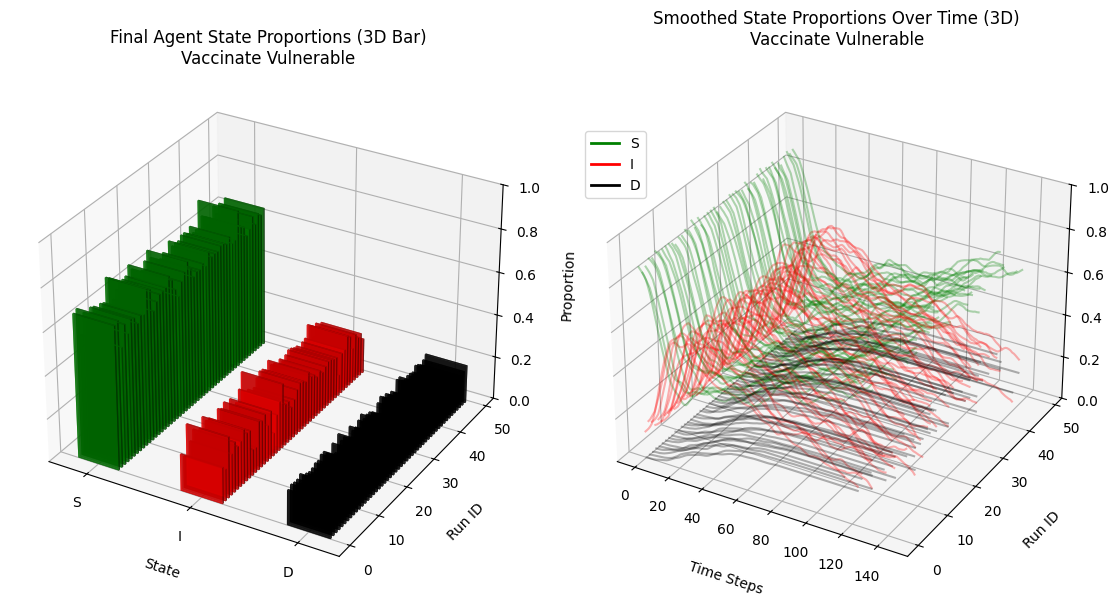
\includegraphics[width=0.95\textwidth]{example_plot.png} % Change filename and width as needed
\caption{Example Simulation: Final and time dependent proportions of agents that were susceptible (green), infected (red) and dead (black). The simulation terminated while there were infected agents, but no new dead registered in the past 50 time steps. The virus aged and the population gained immunity, and therefore it became endemic but relatively harmless due to viral ageing and immunity growth.}
\label{fig:example}
\end{figure}

An anonymised version of the full code, including plots and datasets, is provided at this \href{https://osf.io/mqyhj/?view_only=bccd79641b484abebe18c60bd73cb319}{link}. This will be made publicly available on github if accepted for publication.


\newpage
\begin{table}[h!]
\begin{tabularx}{\textwidth}{|X|X|}
\hline
Simplification & Covid-19\\\hline
Mandatory vaccination strategies apply to the entire population of interest. &Governing bodies had no control over people outside their jurisdiction and infections were imported from abroad \cite{Williams2021}.\\\hline
2 homogeneous sub-populations are stable over time.& Some patients became much more vulnerable due to immunocompromise (e.g., via drugs given to facilitate a transplant or by contracting a disease such as HIV)  \cite{Fung2020}.  Health care workers frequently interacted with vulnerable people and were a vaccination priority \cite{Kelsall2025}. Some people were more likely to spread the virus and thus arguable prime targets for transmission reduction vaccines \cite{rhodes2021justice}.\\\hline
Deterministic evolution to more benign virus variants. & Evolved sub-variants can have greater mortality rates and some mutations are the actual cause of a wave \cite{Kun2023}.\\\hline
The central planner has the authority and capacity to enforce vaccinations.& The was widespread vaccine hesitancy \cite{Yeboah2025}.\\\hline%\cite{Marini2024}
There are no drawbacks of (surviving) an infection. & SARS-CoV-2 infected experienced a lower quality of live and the virus caused long Covid in some \cite{Cutler2022}.\\\hline
Vaccinations only lowers mortality rate, transmission probabilities and recovery time.& Covid vaccines caused nocebo effects \cite{Sever2022a} and rare adverse reactions \cite{Sessa2021}.\\\hline
Vaccination is immediate and not supply constrained. & Vaccine allocation and distribution is a logistical challenge \cite{Muckstadt2023}.\\\hline
The (public) health context stays fixed over time. & Treatment options, health infrastructure (over-crowded hospitals, triage) \cite{Feinstein2020}, public health measures (masks, social distancing, school closures) \cite{Lison2023} and even the weather \cite{Majumder2021} had time varying influences.\\\hline
A single vaccine provides constant health benefits over time.& SARS-CoV-2 mutated \cite{Bruessow2022} and multiple vaccines became available \cite{Li2022b} with time-varying health benefits \cite{Shrestha2024}.\\\hline
Transmission probability and recovery time do not depend on viral age. & In general, ``severe symptoms and higher mortality will often lead to people staying home, reducing the opportunity for the virus to spread.'' \cite[P.\ 6]{Jones2024}\\\hline
\end{tabularx}
\caption{Simplifications of our model compared to Covid-19.}
\label{tab:Simplifications}
\end{table}

\end{document}